\chapter{Construcción de medidas}

\section{Medidas exteriores}

\begin{defi}
    Sea X un conjunto. Una medida exterior sobre X es una aplicación $\mu^*: \mathcal{P}(X) \longrightarrow [0,+\infty]$ tal que
    \begin{enumerate}
        \item[(a)] $\mu^*(\emptyset) = 0$.
        \item[(b)] Si $A \subset B$ entonces $\mu^*(A) \leq \mu^*(B)$.
        \item[(c)] (Subaditividad finita)
              \begin{align*}
                  \mu^*\left(\bigcup_{i=1}^{\infty}{A_i} \right) \leq \sum_{i=1}^{\infty}{\mu^*(A_i)}
              \end{align*}
              para cualquier colección numerable $\{A_i\}_{i=1}^{\infty}$ de subconjuntos de X.
    \end{enumerate}
\end{defi}

\subsection{Construcción de medidas exteriores}

\begin{defi}
    Sea X un conjunto. Decimos que $\mathcal{E}$ es una familia recubridora de X si
    \begin{enumerate}
        \item[(a)] $\mathcal{E} \subset \mathcal{P}(X)$.
        \item[(b)] $\emptyset \in \mathcal{E}$.
        \item[(c)] Existe una colección $\{X_i\}_{i=1}^{\infty}$ de elementos de $\mathcal{E}$ tal que
              $X = \cup_{i=1}^{\infty}{X_i}$.
    \end{enumerate}
\end{defi}

\begin{teo}
    Supongamos que X es un conjunto y que $\mathcal{E}$ es una familia recubridora de X. Sea $\rho: \mathcal{E} \longrightarrow [0,+\infty]$ una aplicación tal que $\rho(\emptyset) = 0$
    \begin{enumerate}
        \item[(a)] Sea $\mu_{\rho}^*: \mathcal{P}(X) \longrightarrow [0,+\infty]$ definida por
              \begin{align*}
                  \mu_{\rho}^*(A) = \inf(H_A)
              \end{align*}
              donde
              \begin{align*}
                  H_A = \left\{ \lambda \in [0,+\infty] : \lambda = \sum_{i=1}^{\infty}{\rho(E_i)} : A \subset \bigcup_{i=1}^{\infty}{E_i}, E_i \in \mathcal{E} \right\}.
              \end{align*}
              Entonces $\mu_{\rho}^*$ es una medida exterior y $\mu_{\rho}^*(A) \leq \rho(A)$ para todo $A \in \mathcal{E}$. (Nótese que el ínfimo de $H_A$ está bien definido y es un elemento de $[0,+\infty]$).
        \item[(b)] Supongamos que, además, la aplicación $\rho$ tiene la propiedad siguiente
              \begin{align*}
                  E \subset \bigcup_{i=1}^{\infty}{E_i}, \ (E, E_i \in \mathcal{E}) \Longrightarrow \rho(E) \leq \sum_{i=1}^{\infty}{\rho(E_i)}.
              \end{align*}
              Entonces $\mu_{\rho}^*$ es una medida exterior tal que $\mu_{\rho}^*(A) = \rho(A)$ para todo $A \in \mathcal{E}$.
    \end{enumerate}
\end{teo}

\begin{proof}
    $(a)$ Observamos primero que $\mu_{\rho}^*$ está bien definida porque cada subconjunto $A$ es recubierto por alguna familia numerable de $\mathcal{E}$ ya que $A \subset X = \cup_{i=1}^{\infty}{X_i}$.

    Antes de probar que $\mu_{\rho}^*$ es una medida exterior, veremos que $\mu_{\rho}^*(A) \leq \rho(A)$ para todo $A \in \mathcal{E}$. Fijado dicho $A$, tomamos la sucesión $\{E_i\}_{i=1}^{\infty}$ definida por $E_1 = A$, $E_i = \emptyset$ para todo $i \ge 2$. Es claro que $A \subset \cup_{i=1}^{\infty}{E_i}$ y que $E_i \in \mathcal{E}$ para todo $i$. Luego $\rho(A) = \rho(E_1) = \sum_{i=1}^{\infty}{\rho(E_i)} \in H_A$ y, por lo tanto,
    \begin{align*}
        \mu_{\rho}^*(A) = \inf(H_A) \leq \rho(A).
    \end{align*}
    Ahora probemos que $\mu_{\rho}^*$ es una medida exterior. Por hipótesis, $\rho(\emptyset) = \sum_{i=1}^{\infty}{\emptyset} = 0 \in H_{\emptyset}$, luego $\mu_{\rho}^*(\emptyset) = 0$. Sean $A, B \in \mathcal{E}$ tales que $A \subset B$, entonces $H_B \subset H_A$, por tanto, $\inf(H_A) \leq \inf(H_B)$, es decir, $\mu_{\rho}^*(A) \leq \mu_{\rho}^*(B)$. Para que $\mu_{\rho}^*$ sea medida exterior solo nos queda probar la subaditividad numerable.

    Fijemos $\varepsilon > 0$. Entonces, para cada $i$, consideramos $\mu_{\rho}^*(A_i) + \frac{\varepsilon}{2^i}$. Como $\mu_{\rho}^*(A_i) = \inf(H_{A_i})$, existe $\lambda_i \in H_{A_i}$ tal que
    \begin{align*}
        \lambda_i \leq \mu_{\rho}^*(A_i) + \frac{\varepsilon}{2^i}.
    \end{align*}
    Como $\lambda_i \in H_{A_i}$, existe una familia numerable $\{E_{ij}\}$, $E_{ij} \in \mathcal{E}$, tal que
    \begin{align*}
        A_i \subset \bigcup_{j=1}^{\infty}{E_{ij}} \ \ y \ \ \lambda_i = \sum_{j=1}^{\infty}{\rho(E_{ij})}.
    \end{align*}
    Es claro que $\cup_{i=1}^{\infty}{A_i} \subset \cup_{i,j=1}^{\infty}{E_{ij}}$. Si $\sigma: \mathbb{N} \longrightarrow \mathbb{N} \times \mathbb{N}$ es una biyección, tenemos que $\{E_{\sigma(k)}\}_{k=1}^{\infty}$ es una colección numerable de elementos de $\mathcal{E}$ tal que $\cup_{i=1}^{\infty}{A_i} \subset \cup_{k=1}^{\infty}{E_{\sigma(k)}} = \cup_{i,j=1}^{\infty}{E_{ij}}$. Por lo tanto, por la definición de $\mu_{\rho}^*$,
    \begin{align*}
        \mu_{\rho}^*\left( \bigcup_{i=1}^{\infty}{A_i}\right) & \leq \sum_{k=1}^{\infty}{\rho(E_{\sigma(k)})} = \sum_{i=1}^{\infty}{\left( \sum_{j=1}^{\infty}{\rho(E_{ij})}\right)}                                                        \\
                                                              & = \sum_{i=1}^{\infty}{\lambda_i} \leq \sum_{i=1}^{\infty}{(\mu_{\rho}^*\left(A_i) + \frac{\varepsilon}{2^i}\right)} = \sum_{i=1}^{\infty}{\mu_{\rho}^*(A_i) + \varepsilon}.
    \end{align*}
    Haciendo que $\varepsilon \to 0^+$ obtenemos
    \begin{align*}
        \mu_{\rho}^*\left( \bigcup_{i=1}^{\infty}{A_i}\right) \leq \sum_{i=1}^{\infty}{\mu_{\rho}^*(A_i)}.
    \end{align*}
    $(b)$ La propiedad añadida a $\rho$ implica trivialmente que $\rho(A) \leq \lambda$ para todo $\lambda \in H_A$ y, en consecuencia, $\rho(A) \leq \mu_{\rho}^*(A)$ para todo $A \in \mathcal{E}$. Por el apartado $(a)$ tenemos la otra desigualdad, luego $\rho(A) = \mu_{\rho}^*(A)$ para todo $A \in \mathcal{E}$.
\end{proof}

\begin{cor}
    La medida exterior de Lebesgue es una medida exterior y $m^*(I) = \mathcal{V}(I)$ para todo intervalo abierto I.
\end{cor}

\subsection{Construcción de medidas: el teorema de Carathéodory}
\begin{teo}
    Supongamos que estamos en las condiciones del teorema anterior. Sea $A \subset X$. Las condiciones siguientes son equivalentes:
    \begin{enumerate}
        \item[(a)] $\mu_{\rho}^*(A \cap E) + \mu_{\rho}^*(A^c \cap E) = \mu_{\rho}^*(E)$ para todo $E \subset X$. \item[(b)] $\mu_{\rho}^*(A \cap E) + \mu_{\rho}^*(A^c \cap E) = \mu_{\rho}^*(E)$ para todo $E \subset \mathcal{E}$.
    \end{enumerate}
\end{teo}

\begin{proof}
    Nótese que solo tenemos que probar $(b) \Longrightarrow (a)$. En primer lugar, por ser $\mu_{\rho}^*$ medida exterior, tenemos
    \begin{align*}
        \mu_{\rho}^*(E) = \mu_{\rho}^*((A \cap E) \cup (A^c \cap E)) \leq \mu_{\rho}^*(A \cap E) + \mu_{\rho}^*(A^c \cap E)
    \end{align*}
    para todo $E \subset X$. Probemos la otra desigualdad. Sea $\{E_i\}_{i=1}^{\infty}$ tal que $E \subset \cup_{i=1}^{\infty}{E_i}$ donde $E_i \in \mathcal{E}$. Entonces
    \begin{align*}
        A \cap E \subset \cup_{i=1}^{\infty}{(A \cap E_i)} \ \ \ y \ \ \ A^c \cap E \subset \cup_{i=1}^{\infty}{(A^c \cap E_i)}.
    \end{align*}
    Aplicamos de nuevo que $\mu_{\rho}^*$ es medida exterior y concluimos que
    \begin{align*}
        \mu_{\rho}^*(A \cap E) \leq \sum_{i=1}^{\infty}{ \mu_{\rho}^*(A \cap E_i)} \ \ \ y \ \ \ \mu_{\rho}^*(A^c \cap E) \leq \sum_{i=1}^{\infty}{ \mu_{\rho}^*(A^c \cap E_i)}.
    \end{align*}
    Sumando ambas desigualdades,
    \begin{align*}
        \mu_{\rho}^*(A \cap E) + \mu_{\rho}^*(A^c \cap E) \leq \sum_{i=1}^{\infty}{( \mu_{\rho}^*(A \cap E_i) + \mu_{\rho}^*(A^c \cap E_i))}.
    \end{align*}
    Aplicando $(b)$, el último término es $\sum_{i=1}^{\infty}{\mu_{\rho}^*(E_i)}$. Luego,
    \begin{align*}
        \mu_{\rho}^*(A \cap E) + \mu_{\rho}^*(A^c \cap E) \leq \sum_{i=1}^{\infty}{\mu_{\rho}^*(E_i)} \leq \sum_{i=1}^{\infty}{\rho(E_i)},
    \end{align*}
    es decir,
    \begin{align*}
        \mu_{\rho}^*(A \cap E) + \mu_{\rho}^*(A^c \cap E) \leq \lambda \ \ \ \forall \lambda \in H_E,
    \end{align*}
    de donde,
    \begin{align*}
        \mu_{\rho}^*(A \cap E) + \mu_{\rho}^*(A^c \cap E) \leq \inf(H_E) = \mu_{\rho}^*(E)
    \end{align*}
    como queríamos demostrar.
\end{proof}

\begin{obs}
    Si tenemos una medida exterior $\mu^*$ arbitraria entonces la afirmación $(b)$ del teorema anterior no tiene sentido porque no existe la familia $\mathcal{E}$. Sin embargo, $(a)$ tiene sentido completo. Por ello, se introduce la siguiente definición.
\end{obs}

\begin{defi}
    Sea $\mu^*$ una medida exterior sobre X. Decimos que $A \subset X$ es un conjunto $\mu^*$-medible (o que A es $mu^*$-medible en el sentido de Carathéodory) si para todo $E \subset X$ se tiene que
    \begin{align*}
        \mu^*(A \cap E) + \mu^*(A^c \cap E) = \mu^*(E),
    \end{align*}
    o, equivalentemente,
    \begin{align*}
        \mu_{E}^*(A) + \mu_{E}^*(A^c) \leq \mu_{E}^*(X).
    \end{align*}
\end{defi}

\begin{obs}
    \begin{enumerate}
        \item[(a)] La desigualdad $\mu^*(A \cap E) + \mu^*(A^c \cap E) \ge \mu^*(E)$ se verifica siempre porque $\mu^*$ es una medida exterior. Luego para probar que $A \subset X$ es un conjunto $\mu^*$-medible basta establecer
              \begin{align*}
                  \mu^*(A \cap E) + \mu^*(A^c \cap E) \leq \mu^*(E)
              \end{align*}
              para todo $E$ con $\mu^*(E) < \infty$.
        \item[(b)] Si $\mu^*(A) = 0$ entonces $A$ es un conjunto $\mu^*$-medible.
              \begin{align*}
                   & A \cap E \subset A \Longrightarrow \mu^*(A \cap E) \leq \mu^*(A) = 0 \Longrightarrow \mu^*(A \cap E) = 0, \\
                   & A^c \cap E \subset E \Longrightarrow \mu^*(A^c \cap E) \leq \mu^*(E).
              \end{align*}
              Sumando estas desigualdades, tenemos que
              \begin{align*}
                  \mu^*(A \cap E) + \mu^*(A^c \cap E) = \mu^*(A^c \cap E) \leq \mu^*(E).
              \end{align*}
    \end{enumerate}
\end{obs}

\begin{teo}[Teorema de Carathéodory]
    Sea $\mu^*$ una medida exterior sobre X y sea
    \begin{align*}
        \mathcal{M}^* = \{ A \subset X : A \ es \ \mu^*\text{-medible} \}.
    \end{align*}
    Entonces
    \begin{enumerate}
        \item[(a)] $\mathcal{M}^*$ es una $\sigma$-álgebra (la $\sigma$-álgebra de Carathéodory).
        \item[(b)] $\mu^*|_{\mathcal{M}^*} = \mu$ es una medida.
        \item[(c)] $(X, \mathcal{M}^*, \mu)$ es un espacio de medida completo.
    \end{enumerate}
\end{teo}

\begin{proof}
    Comenzaremos probando que $\mathcal{M}^*$ es un álgebra.

    Es evidente que $A \in \mathcal{M}^* \Longrightarrow A^c \in \mathcal{M}^*$. Es claro entonces que $X \in \mathcal{M}^*$ puesto que $\emptyset \in \mathcal{M}^*$ ya que $\mu^*(\emptyset) = 0$.

    Supongamos ahora que $A, B \in \mathcal{M}^*$ y demostremos que $A \cup B \in \mathcal{M}^*$. Para ellos, basta usar la subaditividad y la definición de conjunto $\mu^*$-medible (dos veces):
    \begin{align*}
        \mu^*((A \cup B) \cap E) + \mu^*((A \cup B)^c \cap E ) & = \mu^*((A \cup B) \cap E) + \mu^*((A^c \cap B^c \cap E )                    \\
                                                               & = \mu^*((A \cup (B \backslash A)) \cap E) + \mu^*((A^c \cap B^c \cap E )     \\
                                                               & \leq \mu^*(A \cap E) + \mu^*(B \cap A^c \cap E) + \mu^*(B^c \cap A^c \cap E) \\
                                                               & = \mu^*(A \cap E) + \mu^*(A^c \cap E) = \mu^*(E).
    \end{align*}
    Puesto que $\mathcal{M}^*$ es un álgebra, sabemos que si $A, B \in \mathcal{M}^*$ entonces $A^c, A \cup B, A \cap B \in \mathcal{M}^*$.

    Nótese que para todo $E \subset X$, $\mu_E^*(A) = \mu^*(A \cap E)$ es una medida sobre $X$. Veremos que es numerablemente aditiva sobre $\mathcal{M}^*$.

    $(i)$ Comenzamos probando que, para todo $E \subset X$, $\mu_E^*$ es finitamente aditivida sobre $\mathcal{M}^*$, es decir, si $\{A_i\}_{i=1}^{s}$ es una colección finita y disjunta de elementos de $\mathcal{M}^*$, entonces $\mu_E^*(\cup_{i=1}^{s}{A_i}) = \sum_{i=1}^{s}{\mu_E^*(A_i)}$. Por ser $\mathcal{M}^*$ un álgebra, basta verlo para $s = 2$. Sean $A, B \in \mathcal{M}^*$, $A \cap B = \emptyset$.

    Por ser $A \in \mathcal{M}^*$ y $A \cap B = \emptyset$ tenemos que
    \begin{align*}
        \mu_E^*(A \cup B) & = \mu^*((A \cup B) \cap E)                                           \\
                          & = \mu^*((A \cup B)\cap E \cap A) + \mu^*((A \cup B) \cap E \cap A^c) \\
                          & = \mu^*(A \cap E) + \mu^*(B \cap E) = \mu_E^*(A) + \mu_E^*(B).
    \end{align*}
    $(ii)$ Vamos a probar ahora que, para todo $E \subset X$, $\mu_E^*$ es numerablemente aditiva sobre $\mathcal{M}^*$, es decir,  si $\{A_i\}_{i=1}^{\infty}$ es una colección numerable y disjunta de elementos de $\mathcal{M}^*$, entonces $\mu_E^*(\cup_{i=1}^{\infty}{A_i}) = \sum_{i=1}^{\infty}{\mu_E^*(A_i)}$.

    Por la subaditividad numerable de la medida exterior $ \mu_E^*$,
    \begin{align*}
        \mu_E^*(\cup_{i=1}^{\infty}{A_i}) \leq \sum_{i=1}^{\infty}{\mu_E^*(A_i)}.
    \end{align*}
    Por ser $ \mu_E^*$ finitamente aditiva sobre $\mathcal{M}^*$ y por ser una medida exterior,
    \begin{align*}
        \sum_{i=1}^{N}{\mu_E^*(A_i)} = \mu_E^*(\cup_{i=1}^{N}{A_i}) \leq \mu_E^*(\cup_{i=1}^{\infty}{A_i}).
    \end{align*}
    Tomando límite $N \to \infty$, llegamos a que
    \begin{align*}
        \sum_{i=1}^{\infty}{\mu_E^*(A_i)}  \leq \mu_E^*(\cup_{i=1}^{\infty}{A_i}).
    \end{align*}
    Por consiguiente, $\mu_E^*(\cup_{i=1}^{\infty}{A_i}) = \sum_{i=1}^{\infty}{\mu_E^*(A_i)}$, como queríamos demostrar.

    $(iii)$ Del punto anterior, tomando $E = X$, tenemos que si $\{A_i\}_{i=1}^{\infty}$ es una colección numerable y disjunta de elementos de $\mathcal{M}^*$, entonces
    \begin{align*}
        \mu^*(\cup_{i=1}^{\infty}{A_i}) = \sum_{i=1}^{\infty}{\mu^*(A_i)}.
    \end{align*}
    Una vez que sabemos que $\mathcal{M}^*$ es un álgebra, estableceremos que es cerrada para uniones numerables y disjuntasm es decir, vamos a probar que

    $(iv)$ si $\{A_i\}_{i=1}^{\infty}$ es una sucesión tal que $A_i \in \mathcal{M}^*$, $A_i \cap A_j = \emptyset$ si $i \not = j$ entonces
    \begin{align*}
        B = \cup_{i=1}^{\infty}{A_i} \in \mathcal{M}^*.
    \end{align*}
    Sea $B_n = \cup_{i=1}^{N}{A_i}$. Por ser $\mathcal{M}^*$ un álgebra, ya sabemos que $B_n \in \mathcal{M}^*$. Además si $E \subset X$
    \begin{align*}
        \mu_E^*(B) & = \mu_E^*(\cup_{i=1}^{\infty}{A_i}) = \sum_{i=1}^{\infty}{\mu_E^*(A_i)}                                                                       \\
                   & = \lim_{N \to \infty}{ \sum_{i=1}^{N}{\mu_E^*(A_i)}} = \lim_{N \to \infty}{\mu_E^*(\cup_{i=1}^{N}{A_i})} = \lim_{N \to \infty}{\mu_E^*(B_n)}.
    \end{align*}
    Así,
    \begin{align*}
        \mu_E^*(B) + \mu_E^*(B^c) = \lim_{N \to \infty}{(\mu_E^*(B_n) + \mu_E^*(B^c))}.
    \end{align*}
    Por otra parte, como $B_n \subset B$ tenemos que $B^c \subset B_n^c$. Luego
    \begin{align*}
        \mu_E^*(B^c) \leq \mu_E^*(B_n^c)
    \end{align*}
    para todo n. Puesto que $\mu_E^*$ es una medida exterior y $B_n \in \mathcal{M}^*$,
    \begin{align*}
        \mu_E^*(B_n) + \mu_E^*(B^c) \leq \mu_E^*(B_n) + \mu_E^*(B_n^c) = \mu^*(E).
    \end{align*}
    Por lo tanto,
    \begin{align*}
        \mu_E^*(B) + \mu_E^*(B^c)  = \lim_{N \to \infty}{(\mu_E^*(B_n) + \mu_E^*(B^c))} \leq \mu^*(E).
    \end{align*}
    lo que prueba que $B \in \mathcal{M}^*$.

    $(v)$ Veamos que $\mathcal{M}^*$ es una $\sigma$-álgebra. Tomemos $\{E_i\}_{i=1}^{\infty}$, $E_i \in \mathcal{M}^*$. Si $A_1 = E_1$ y $A_i = E_i \backslash \cup_{n=1}^{i-1}{E_n}$, $i > 1$, se tiene que $A_i \in \mathcal{M}^*$ (por ser $\mathcal{M}^*$ un álgebra), $cup_{i=1}^{\infty}{E_i} = \cup_{i=1}^{\infty}{A_i}$ y los $A_i$ son disjuntos. Por lo ya probado, se sigue que $\cup_{i=1}^{\infty}{E_i} \in \mathcal{M}^*$.

    $(vi)$ Pasamos a demostrar que $\mu^*|_{\mathcal{M}^*} = \mu$ es una medida. Es obvio que $\mu(\emptyset) = 0$. Por $(iii)$, $\mu^*$ es numerablemente aditivda sobre $\mathcal{M}^*$.

    $(vii)$ Nos queda ver que $\mu$ es completa pero esto es obvio: si $\mu(N) = 0$ y $F \subset N$ entonces $\mu^*(F) \leq \mu^*(N) = \mu(N) = 0$; luego $\mu^*(F) = 0$ y, en consecuencia, $F \in \mathcal{M}^*$.
\end{proof}

\section{La medida de Lebesgue}

Definimos la medida exterior de Lebesgue $m^*: \mathcal{P}(\mathbb{R}^n) \longrightarrow [0,+\infty]$ como
\begin{align*}
    m^*(A) = \inf \left\{ \sum_{i=1}^{\infty}{\mathcal{V}(I_i)} : A \subset \cup_{i=1}^{\infty}{I_i}, I_i \text{ es un intervalo de } \mathbb{R}^n\right\}
\end{align*}
La familia $\mathcal{E}$ de los intervalos abiertos es una familia recubridora de $\mathbb{R}^n$ y la aplicación
\begin{align*}
    \rho : \mathcal{E} \longrightarrow [0,+\infty], \ \ \ \rho(I) = \mathcal{V}(I),
\end{align*}
cumple que $\rho(\emptyset) = 0$. Por el teorema de construcción de medidas exteriores, $m^*$ es una medida exterior. Además, si $I \subset \cup_{j=1}^{\infty}{I_j}$ donde $I$ y los $I_j$ son intervalos abiertos, se tiene que
\begin{align*}
    \rho(I) = \mathcal{V}(I) \leq \sum_{j=1}^{\infty}{\mathcal{V}(I_j)} = \sum_{j=1}^{\infty}{\rho(I_j)}.
\end{align*}
Luego, por el apartado $(b)$ del mismo teorema, $m^*(I) = \mathcal{V}(I)$ para todo intervalo abierto.

Obsérvese que $m^*(A) = 0$ si y solo si para todo $\varepsilon > 0$ existe una familia numerable de intervalos abiertos $\{I_i\}_{i=1}^{\infty}$ tal que
\begin{align*}
    A \subset \cup_{i=1}^{\infty}{I_i} \ \ \ y \ \ \ \sum_{j=1}^{\infty}{\mathcal{V}(I_i)} < \varepsilon.
\end{align*}
Recordemos que, por el teorema de Carathéodory,
\begin{align*}
    \mathcal{L} & = \{A \subset \mathbb{R}^n : A \ es \ m^* \text{-medible} \}                                                       \\
                & = \{A \subset \mathbb{R}^n : m^*(A \cap E) + m^*(A^c \cap E) = m^*(E) \text{ para todo } E \subset \mathbb{R}^n \}
\end{align*}
es una $\sigma$-álgebra.

Como $m^*$ viene definida a través de $\rho = \mathcal{V}$ y la familia elemental de los intervalos abiertos, resulta que
\begin{align*}
    \mathcal{L} = \{A \subset \mathbb{R}^n : m^*(A \cap E) + m^*(A^c \cap E) = m^*(E) \text{ para todo intervalo abierto } I\}
\end{align*}
A $\mathcal{L}$ la llamaremos $\sigma$-álgebra de Lebesgue. A los conjuntos $A \in \mathcal{L}$ los llamaremos conjuntos medibles-Lebesgue. Además, por el teorema de Carathéodory, si $m = m^*|_{\mathcal{L}}$ entonces $(\mathbb{R}^n, \mathcal{L}, m)$ es un espacio de medida completo. A $m$ le llamamos la medida de Lebesgue.

\begin{prop}
    Algunas propiedades de $m^*$, $m$ y $\mathcal{L}$.
    \begin{enumerate}
        \item[(a)] Si $m^*(A) = 0$ entonces $A \in \mathcal{L}$.
        \item[(b)] La medida exterior de un intervalo I es  su volumen.
        \item[(c)] $m^*(\{x\}) = 0$ para todo $x \in \mathbb{R}^n$.
        \item[(d)] La medida exterior de Lebesgue de un conjunto numerable A es cero, por lo tanto, $A \in \mathcal{L}$.
        \item[(e)] La medida exterior de $\mathbb{R}^n$ es $+\infty$.
        \item[(f)] La medida exterior es invariante frente a traslaciones: si $A \subset \mathbb{R}^n$ y $b \in \mathbb{R}^n$ entonces $m^*(A + b) = m^*(A)$, donde
              \begin{align*}
                  A + b = \{ x : x = a + b, a \in A \}.
              \end{align*}
        \item[(g)] Para cada $a \in \mathbb{R}$ y para cada $j \in \{1,..., n \}$ los conjuntos
              \begin{itemize}
                  \item $\{x \in \mathbb{R}^n : x = (x_1,...,x_n), x_j > a\}$.
                  \item $\{x \in \mathbb{R}^n : x = (x_1,...,x_n), x_j \leq a\}$.
                  \item $\{x \in \mathbb{R}^n : x = (x_1,...,x_n), x_j \ge a\}$.
                  \item $\{x \in \mathbb{R}^n : x = (x_1,...,x_n), x_j < a\}$.
              \end{itemize}
              son medibles Lebesgue.
        \item[(h)] Los intervalos I son medibles Lebesgue y $m(I) = \mathcal{V}(I)$.
        \item[(i)] $\mathcal{B}_{\mathbb{R}^n} \subset \mathcal{L}$ (los borelianos son medibles Lebesgue).
        \item[(j)] $(\mathbb{R}^n, \mathcal{L}, m)$ es un espacio de medida $\sigma$-finito o, en otras palabras, la medida de Lebesgue es $\sigma$-finita.
    \end{enumerate}
\end{prop}

\begin{proof}
    Probemos $(g)$. Lo veremos solo para $A = \{x \in \mathbb{R}^n : x = (x_1,...,x_n), x_1 > a\}$. Sea $I = (a_1,b_1)\times ... \times (a_n,b_n)$ intervalo abierto. Tenemos tres posibilidad:
    \begin{enumerate}
        \item[(i)] $a_1 \ge a$. Entonces $I \subset A$. Además, $m^*(A \cap I) + m^*(A^c \cap I) = m^*(A \cap I) = m^*(I)$.
        \item[(ii)] $b_j \leq a$. Entonces $I \subset A^c$. Así, $m^*(A \cap I) + m^*(A^c \cap I) = m^*(A \cap I) = m^*(I)$.
        \item[(iii)] $a_j < a < b_j$. Entonces
              \begin{align*}
                   & A \cap I = (a_1,b_1) \times ... \times (a_n,b_n) \text{ y } \\
                   & A^c \cap I =  (a_1,a] \times ... \times (a_n,b_n).
              \end{align*}
              Como estos conjuntos son intervalos,
              \begin{align*}
                   & m^*(A \cap I) = (b_1 - a_1) \dotsb (b_n - a_n) \text{ y } \\
                   & m^*(A^c \cap I) = (a - a_1) \dotsb (b_n - a_n).
              \end{align*}
              de donde
              \begin{align*}
                  m^*(A \cap I) + m^*(A^c \cap I) = \frac{(b_1 - a_1)\dotsb (b_n - a_n)}{(b_1 - a_1)}(b_1 - a + a - a_1) = \mathcal{V}(I) = m^*(I).
              \end{align*}
    \end{enumerate}
\end{proof}

\newpage
\section{Conjuntos medibles Lebesgue y la medida de Lebesgue: caracterizaciones}

\begin{teo}
    Sea $A \subset \mathbb{R}^n$. Las afirmaciones siguientes son equivalentes:
    \begin{enumerate}
        \item[(a)] A es medible-Lebesgue.
        \item[(b)] Para cada $\varepsilon > 0$ existe un abierto G tal que $A \subset G$ y $m^*(G \backslash A) < \varepsilon$.
        \item[(c)] Existen una familia numerable de conjuntos abiertos $\{G_i\}_{i=1}^{\infty}$ y un conjunto N de medida cero tales que $A = (\cap_{i=1}^{\infty}{G_i}) \backslash N$.
    \end{enumerate}
\end{teo}

\begin{proof}
    $(a) \Longrightarrow (b)$ Supongamos que $m(A) < +\infty$. Sea $\varepsilon > 0$. Por la definición de $m = m^*|_{\mathcal{L}}$, existe $\{I_j\}_{j=1}^{\infty}$, un recubrimiento de $A$ por intervalos abiertos, con $\sum_{j=1}^{\infty}{\mathcal{V}(I_J)} < m(A) + \varepsilon$. Tomemos $G = \cup_{j=1}^{\infty}{I_j}$. Así, $G$ es abierto y $A \subset G$. Además,
    \begin{align*}
        m^*(G \backslash A) & = m(G \backslash A) = m(G) - m(A) = m(\cup_{j=1}^{\infty}{I_j}) -  m(A)                               \\
                            & \leq \sum_{j=1}^{\infty}{m(I_j)} - m(A) = \sum_{j=1}^{\infty}{\mathcal{V}(I_j)} - m(A) < \varepsilon.
    \end{align*}
    Supongamos que $m(A) = +\infty$. Sea, para cada $k \in \mathbb{N}$, $I_k = [-k,k]^n$. Así,
    \begin{align*}
        A = A \cap \mathbb{R}^n = \bigcup_{k=1}^{\infty}{A \cap I_k} = \bigcup_{k=1}^{\infty}{A_k},
    \end{align*}
    donde $A_k = A \cap I_k$. Para todo $k \in \mathbb{N}$, $A_k$ es medible y con medida finita ($m(A) \leq m(I_k) < +\infty$). Por lo que hemos demostrado anteriormente, para cada $k \in \mathbb{N}$, existe un abierto $G_k$ con $A_k \subset G_k$ y tal que $m^*(G_k \backslash A_k) < \frac{\varepsilon}{2^k}$. Sea $G = \cup_{k=1}^{\infty}{G_k}$. Es claro que $G$ es abierto y $A \subset G$. Además,
    \begin{align*}
        G \backslash A = \left( \bigcup_{k=1}^{\infty}{G_k} \backslash \bigcup_{k=1}^{\infty}{A_k} \right) \subset \bigcup_{k=1}^{\infty}{(G_k \backslash A_k)}.
    \end{align*}
    Aplicando las propiedades de la medida exterior,
    \begin{align*}
        m^*(G \backslash A) \leq m^*\left(  \bigcup_{k=1}^{\infty}{(G_k \backslash A_k)} \right) \leq \sum_{k=1}^{\infty}{m^*(G_k \backslash A_k)} \leq \sum_{k=1}^{\infty}{\frac{\varepsilon}{2^k}} = \varepsilon.
    \end{align*}
    $(b) \Longrightarrow (c)$ Por hipótesis, para todo $k \in \mathbb{N}$, existe un abierto $G_k$ tal que $A \subset G_k$ y con $m^*(G_k \backslash A) < \frac{1}{k}$. Sea $G = \cap_{k=1}^{\infty}{G_k}$. Entonces $A \subset G$. Por lo tanto, $G \backslash A \subset G_k \backslash A$ para todo $k \in \mathbb{N}$, y, consecuentemente,
    \begin{align*}
        m^*(G \backslash A) < \frac{1}{k} \ \ \text{para todo } k \in \mathbb{N}.
    \end{align*}
    Tomando límite, obtenemos que $m^*(G \backslash A) = 0$, lo que implica que $N = G \backslash A$ es medible y $m(N) = 0$. Por otra parte, $G \backslash N = G \backslash (G \backslash A) = A$.

    $(c) \Longrightarrow (a)$ Es trivial. Por hipótesis, se tiene que $\cap_{i=1}^{\infty}{G_k} \in \mathcal{L}$ y $N \in \mathcal{L}$, por tanto, $A = (\cap_{i=1}^{\infty}{G_k}) \backslash N \in \mathcal{L}$.
\end{proof}

\begin{teo}
    Sea $A \subset \mathbb{R}^n$. Las afirmaciones siguientes son equivalentes:
    \begin{enumerate}
        \item[(a)] A es medible-Lebesgue.
        \item[(b)] Para cada $\varepsilon > 0$ existe un cerrado F tal que $F \subset A$ y $m^*(A \backslash F) < \varepsilon$.
        \item[(c)] Existen una familia numerable de cerrados $\{F_i\}_{i=1}^{\infty}$ y un conjunto N de medida cero tales que $A = (\cup_{i=1}^{\infty}{F_i}) \cup N$.
    \end{enumerate}
\end{teo}

\begin{proof}
    $(a) \Longrightarrow (b)$ Sea $\varepsilon > 0$. Como $A$ es medible, tenemos que $A^c$ es medible. Por el teorema anterior, existe un abierto $G$ tal que $A^c \subset G$ y $m^*(G \backslash A^c) < \varepsilon$. Sea $F = G^c$. Es claro que $F$ es cerrado y $F = G^c \subset A$. Además, $A \backslash F = A \cap F^c = A \cap G = G \backslash A^c$. Por consiguiente,
    \begin{align*}
        m^*(A \backslash F) = m^*(G \backslash A^c) < \varepsilon.
    \end{align*}
    $(b) \Longrightarrow (a)$ Sea $\varepsilon > 0$. Entonces, por hipótesis, existe un cerrado $F \subset A$ tal que $m^*(A \backslash F) < \varepsilon$, de donde, $A^c \subset  F^c$ y $m^*(F^c \backslash A^c) < \varepsilon$ (ya que $F^c \backslash A^c = F^c \cap (A^c)^c = F^c \cap A = A \backslash F$). Tomando $G = F^c$, se tiene que $A^c \subset G$, $G$ es abierto y $m^*(G \backslash A^c) < \varepsilon$. Entonces, por el teorema anterior, $A^c$ es medible-Lebesgue y, consecuentemente, $A$ es medible-Lebesgue.

    $(a) \Longrightarrow (c)$ Supongamos que $A$ es medible-Lebesgue. Entonces $A^c$ es medible. Por el teorema anterior, existe una familia numerable de abiertos $\{G_j\}_{j=1}^{\infty}$ y un conjunto $N$ tales que $m(N) = 0$ y $A^c = (\cap_{j=1}^{\infty}{G_j}) \backslash N$. Entonces
    \begin{align*}
        A^c = \left( \bigcap_{j=1}^{\infty}{G_j}\right) \backslash N = \bigcap_{j=1}^{\infty}{G_j \cap N^c}
    \end{align*}
    o, equivalentemente,
    \begin{align*}
        A = \left( \bigcup_{j=1}^{\infty}{G_j^c}\right) \cup N.
    \end{align*}
    Lo que prueba la implicación ya que los conjuntos $G_j^c$ son cerrados y $m(N) = 0$.

    $(c) \Longrightarrow (a)$ Es trivial. Por hipótesis, se tiene que $\cup_{i=1}^{\infty}{F_k} \in \mathcal{L}$ y $N \in \mathcal{L}$, por tanto, $A = (\cup_{i=1}^{\infty}{F_k} )\cup N \in \mathcal{L}$.
\end{proof}

\begin{cor}
    Un conjunto $A \subset \mathbb{R}^n$ es medible-Lebesgue si y solo si existen un conjunto de Borel B y un conjunto F de medida cero tal que $A = B \cup F$.
\end{cor}

\begin{proof}
    $\Longrightarrow$ Sea $N \in \mathcal{B}_{\mathbb{R}^n}$ con $m(N) = 0$. Entonces
    \begin{align*}
        m^*(F) \leq m^*(N) = m(N) = 0,
    \end{align*}
    por tanto, $m^*(F) = 0$, luego, $F$ es medible-Lebesgue.

    $\Longleftarrow$ Sea $F \in \mathcal{L}$ con $m(F) = 0$. Como $F$ es medible-Lebesgue, existen una familia numerable de conjuntos abiertos $\{G_i\}_{i=1}^{\infty}$ y un conjunto N de medida cero tales que $F = (\cap_{i=1}^{\infty}{G_i}) \backslash N$, por tannton $N \subset \cap_{i=1}^{\infty}{G_i}$, luego, $F \subset \cap_{i=1}^{\infty}{G_i} \in \mathcal{B}_{\mathbb{R}^n}$. Sea $B = F \cup N$, entonces $B$ es medida cero, pues es unión de dos conjuntos de medida cero.
\end{proof}

\begin{cor}
    El espacio de medida de Lebesgue $(\mathbb{R}^n, \mathcal{L}, m)$ es la completación del espacio de medida $(\mathbb{R}^n, \mathcal{B}_{\mathbb{R}^n}, m|_{\mathcal{B}_{\mathbb{R}^n}})$.
\end{cor}

\begin{proof}
    Consideremos el espacio de medida $(\mathbb{R}^n, \mathcal{L}, m)$, donde $\mathcal{L}$ es la $\sigma$-álgebra de Lebesgue y $m$ es la medida de Lebesgue.

    Como $\mathcal{B}_{\mathbb{R}^n} \subset \mathcal{L}$, se tiene que $(\mathbb{R}^n, \mathcal{B}_{\mathbb{R}^n}, \mu)$ es un espacio de medida, donde $\mu =  m|_{\mathcal{B}_{\mathbb{R}^n}}$. Además,
    \begin{align*}
        \mathcal{L} & = \{ A \subset \mathbb{R}^n : A = E \cup F, E \in \mathcal{B}_{\mathbb{R}^n}, F \in \mathcal{L}, m(F) = 0\}                          \\
                    & = \{ A \subset \mathbb{R}^n : A = E \cup F, E \in \mathcal{B}_{\mathbb{R}^n}, F \subset N \in \mathcal{B}_{\mathbb{R}^n}, m(N) = 0\} \\
                    & = \overline{\mathcal{B}_{\mathbb{R}^n}}.
    \end{align*}
    Por otra parte, si $A \in \mathcal{L}$, $A = E \cup F$, $E \in \mathcal{B}_{\mathbb{R}^n}$, $F \subset N \in \mathcal{B}_{\mathbb{R}^n}$, $m(N) = 0$, entonces
    \begin{align*}
        \overline{\mu}(A) = \mu(E) = m(E).
    \end{align*}
    y
    \begin{align*}
        m(A) = m(E \cup F) \leq m(E) + m(F) = m(E) \leq m(A).
    \end{align*}
    Luego, $\overline{\mu}(A) = m(A)$.
\end{proof}

\begin{teo}
    Si $A \subset \mathbb{R}^n$ es un conjunto medible entonces
    \begin{align*}
        m(A) & = \inf{\{ m(G) : A \subset G, G \ abierto \ de \ \mathbb{R}^n \}} \\
             & = \sup{\{ m(K) : K \subset A, K \ compacto \ de \mathbb{R}^n \}}
    \end{align*}
\end{teo}

\begin{teo}[La medida de Lebesgue es invariante frente a traslaciones]
    Sean $A \subset \mathbb{R}^n$ y $b \in \mathbb{R}^n$. A es un conjunto medible si y solo si A + b es medible y, en este caso, $m(A + b) = m(A)$.
\end{teo}

\begin{proof}
    Definimos $T_b: \mathbb{R}^n \longrightarrow \mathbb{R}^n$ dada por $T_b(x) = x + b$, que es biyectiva. Ya sabemos que $m^*(T_bE) = m^*(E + b) = m^*(E)$ para todo conjunto $E$. Basta demostrar que si $A$ es un conjunto medible-Lebesgue entonces $A + b$ es medible y, en este caso, $m(A + b) = m(A)$. Supongamos que $A$ es medible. Sea $\varepsilon > 0$. Por ser $A$ medible, existe un abierto $G$ tal que $A \subset G$ y $m(G \backslash A) < \varepsilon$. Como $T_b$ es un homeomorfismo, $T_bG$ es un abierto y, además, $T_bA \subset T_bG$. Como $T_bG \backslash T_bA = T_b(G \backslash A)$ y $m^*$ es invariante frente a traslaciones, resulta que
    \begin{align*}
        m^*(T_bG \backslash T_bA) = m^*(T_b(G \backslash A)) = m^*(G \backslash A) < \varepsilon.
    \end{align*}
    Por lo tanto, $T_bA$ es medible y $m(T_bA) = m^*(T_bA) = m(A)$.
\end{proof}

\section{Cubos diádicos y conjuntos abiertos}

\begin{defi}
    Un intervalo diádico de longitud $2^{-k}$ en $\mathbb{R}$ es un intervalo de la forma $I = (m2^{-k}, (m+1)2^{-k}]$, con $m,k \in \mathbb{Z}$.
\end{defi}

\begin{obs}
    Algunas propiedades inmediatas son
    \begin{enumerate}
        \item[1.] Fijado $k \in \mathbb{Z}$, los intevalos $2^{-k}$ constituyen una partición numerable de $\mathbb{R}$.
        \item[2.] Dados dos intervalos diádicos de longitud $2^{-k}$, $k \in \mathbb{Z}$, se tiene que, o son iguales o son disjuntos.
        \item[3.] Dados dos intervalos diádicos cualesquiera, o bien son disjuntos, o bien uno está contenido en el otro.
    \end{enumerate}
\end{obs}

\begin{defi}
    Un cubo diádico de $\mathbb{R}^n$ de lado $2^{-k}$, con $k \in \mathbb{Z}$, es un producto cartesiano de n intervalos diádicos de $\mathbb{R}$ de longitud $2^{-k}$, es decir, es de la forma
    \begin{align*}
        I = (m_12^{-k}, (m_1 + 1)2^{-k}] \times ... \times (m_n2^{-k}, (m_n + 1)2^{-k}], \ \ \ \ m_j \in \mathbb{Z}.
    \end{align*}
    Denotaremos por $\mathcal{D}_k$ a la familia de los cubos diádicos en $\mathbb{R}^n$ de lado $2^{-k}$, mientras que $\mathcal{D}$ será la unión $\cup_{k \in \mathbb{Z}}{\mathcal{D}_k}$, esto es, $\mathcal{D}$ es la familia de todos los cubos diádicos de $\mathbb{R}^n$.
\end{defi}

\begin{teo}
    Sea $G = \emptyset$ un abierto de $\mathbb{R}^n$. Entonces existe una familia numerable $\{I_j\}$ de cubos diádicos disjuntos tal que $G = \cup_{j}{I_j}$.
\end{teo}

\begin{teo}
    Sea $E \subset \mathbb{R}^n$ medible y de medida finita. Para todo $\varepsilon > 0$ existe una colección finita $\{Q_j\}_{j=1}^{N}$ de cubos cerrados disjuntos tal que si $F = \cup_{j=1}^{N}{Q_j}$ se tiene que $m(E \bigtriangleup F) < \varepsilon$. ($E \bigtriangleup F = (E \backslash F) \cup (F \backslash E))$.
\end{teo}

\section{Funciones simples en $\mathbb{R}^n$}

\begin{defi}
    Una función paso $\varphi$ es una combinación lineal finita de funciones características de rectángulos (intervalos acotados), es decir,
    \begin{align*}
        \varphi = \sum_{i=1}^{s}{a_i\mathcal{X}_{R_i}},
    \end{align*}
    donde $a_i \in \mathbb{R}$ y $R_i$ es un rectángulo.
\end{defi}

\begin{teo}
    Si $f: \mathbb{R}^n \longrightarrow \mathbb{R}$ es una función medible, entonces existe una sucesión $\{\varphi_k\}$ de funciones paso que converge a f en casi todo punto de $\mathbb{R}^n$.
\end{teo}

\section{Relación entre las medidas de Lebesgue}

\begin{teo}
    Consideramos $(\mathbb{R}^p, \mathcal{L}_p, m_p)$ y $(\mathbb{R}^q, \mathcal{L}_q, m_q)$ los espacios de medida de Lebesgue de $\mathbb{R}^p$ y $\mathbb{R}^q$, respectivamente. Si A es medible en $\mathbb{R}^p$ ($A \in \mathcal{L}_p$) y B es medible en $\mathbb{R}^q$ ($B \in \mathcal{L}_q$) entonces $A \times B$ es medible en $\mathbb{R}^{p + q}$ ($A \times B \in \mathcal{L}_{p + q}$) y $m_{p + q}(A \times B) = m_p(A)m_q(B)$.
\end{teo}

\section{La medida de Lebesgue-Stieltjes en $\mathbb{R}$}

Las funciones crecientes y continuas por la derecha se denominan funciones de distribución. A cada función de distribución $F$ le vamos a asignar una medida de Borel en $\mathbb{R}$, es decir, una medida definida en la $\sigma$-álgebra de Borel tal que la medida del intevalo $(a,b]$ es $F(b) - F(a)$. Es de destacar que solo existe una medida con estas propiedades.

\begin{teo}
    Sea $F: \mathbb{R} \longrightarrow \mathbb{R}$ una función creciente continua por la derecha (una función de distribución). Entonces existe una única medida $m_F$ definida sobre $\mathcal{B}_{\mathbb{R}}$ tal que $m_F((a,b]) = F(b) - F(a)$ para todo intervalo $(a,b]$, $a,b \in \mathbb{R}$, $a \leq b$. Dicha medida recibe el nombre de medida de Lebesgue-Stieltjes asociada a $F$. Si $F$ es la función identidad, $F(x) = x$, $m_F$ es la medida de Lebesgue (es la única medida $m$ definida sobre $\mathcal{B}_{\mathbb{R}}$ tal que $m((a,b]) = b - a$).
\end{teo}

\begin{itemize}
    \item \textbf{Existencia}. Sea $\mathcal{E} = \{ (a,b] : a,b \in \mathbb{R}, a \leq b \}$. Definamos $\rho : \mathcal{E} \longrightarrow [0,+\infty)$ como $\rho((a,b]) = F(b) - F(a)$. $\mathcal{E}$ es una familia recubridora de $\mathbb{R}$ pues
          \begin{itemize}
              \item $\emptyset = (a,a] \in \mathcal{E}$ y
              \item $\mathbb{R} = \cup_{n=1}^{\infty}(-n,n]$.
          \end{itemize}
          Además, $\rho(\emptyset) = \rho((a,a]) = F(a) - F(a) = 0$, independientemente del $a$ elegido. Luego, por el teorema de construcción de medidas exteriores, $m_F^*: \mathcal{P}(\mathbb{R}) \longrightarrow [0,+\infty]$ definida por
          \begin{align*}
              m_F^*(A) = \inf \left\{ \sum_{i=1}^{\infty}{\rho(E_i)} : A \subset \cup_{i=1}^{\infty}{(a_i,b_i]}, (a_i,b_i] \in \mathcal{E} \right\}
          \end{align*}
          es una medida exterior. Sea
          \begin{align*}
              \mathcal{M}_F^* & = \{ A \subset \mathbb{R} : m_F^*(A \cap E) + m_F^*(A^c \cap E) = m_F^*(E) \text{ para todo } E \subset \mathbb{R} \}              \\
                              & = \{ A \subset \mathbb{R} : m_F^*(A \cap (a,b]) + m_F^*(A^c \cap (a,b]) = m_F^*((a,b]) \text{ para todo } (a,b] \in \mathcal{E} \}
          \end{align*}
          la $\sigma$-álgebra de Carathéodory asociada a $m_F^*$. Se tienen las propiedades siguientes
          \begin{itemize}
              \item $m_F^*((a,b]) = F(b) - F(a)$, $a \leq b$, $a,b \in \mathbb{R}$. Para probar esta propiedad, hacemos uso del siguiente lema
                    \begin{lema}
                        Si $(a,b] \subset \cup_{i=1}^{\infty}{(a_i,b_i]}$ entonces
                        \begin{align*}
                            \rho((a,b]) = F(b) - F(a) \leq \sum_{i=1}^{\infty}(F(b_i) - F(a_i)).
                        \end{align*}
                    \end{lema}
              \item Es importante el siguiente lema.
                    \begin{lema}
                        Todo intervalo semiabierto $(-\infty,c]$ es $m_F^*$-medible.
                    \end{lema}
                    \begin{proof}
                        Sea $(a,b] \in \mathcal{E}$, entonces
                        \begin{enumerate}
                            \item[(i)] Si $c \leq a$
                                  \begin{align*}
                                       & (-\infty,c] \cap (a,b] = \emptyset                         \\
                                       & (-\infty,c]^c \cap (a,b] = (c,+\infty) \cap (a, b] = (a,b]
                                  \end{align*}
                                  por tanto, $m_F^*((-\infty,c] \cap (a,b]) + m_F^*( (-\infty,c]^c \cap (a,b]) = m_F^*((a,b])$.
                            \item[(ii)] Si $c \ge b$
                                  \begin{align*}
                                       & (-\infty,c] \cap (a,b] = (a,b]                                 \\
                                       & (-\infty,c.]^c \cap (a,b] = (c,+\infty) \cap (a,b] = \emptyset
                                  \end{align*}
                                  por tanto, $m_F^*((-\infty,c] \cap (a,b]) + m_F^*( (-\infty,c]^c \cap (a,b]) = m_F^*((a,b])$.
                            \item[(iii)] Si $a < c < b$
                                  \begin{align*}
                                       & (-\infty,c] \cap (a,b] = (a,c]                             \\
                                       & (-\infty,c]^c \cap (a,b] = (c, +\infty) \cap (a,b] = (c,b]
                                  \end{align*}
                                  por tanto, $m_F^*((-\infty,c] \cap (a,b]) + m_F^*( (-\infty,c]^c \cap (a,b]) = m_F^*((a,b])$.
                        \end{enumerate}
                    \end{proof}
              \item El lema anterior demuestra que $\mathcal{B}_{\mathbb{R}} \subset \mathcal{M}_F^*$ ya que $\mathcal{M}_F^*$ es una $\sigma$-álgebra y los intervalos $(-\infty,c]$ generan la $\sigma$-álgebra de Borel de $\mathbb{R}$.
              \item $m_F = m_F^* |_{\mathcal{M}_F^*}$ es completa (por el Teorema de Carathéodory).
              \item Es claro que $m_F = m_F^* | _{\mathcal{B}_{\mathbb{R}}}$ cumple las condiciones requeridas.
          \end{itemize}
    \item \textbf{Unicidad}: Solo nos interesa saber que es única, la demostración se deja como ejercicio.

          El resultado siguiente es un recíproco de lo que hemos demostrado.
          \begin{teo}
              Si $\mu$ es una medida de Borel sobre $\mathbb{R}$ que es finita para todo intervalo acotado, entonces existe $F: \mathbb{R} \longrightarrow \mathbb{R}$ creciente y continua por la derecha tal que $m_F = \mu$.
          \end{teo}
          \begin{proof}
              Definimos
              \begin{align*}
                  F(x) = \left\{ \begin{array}{lcc}
                                     -\mu((x,0]) & si & x \leq 0 \\
                                     \mu((0,x])  & si & x > 0    \\
                                 \end{array}
                  \right.
              \end{align*}
              $F$ cumple las condiciones.
          \end{proof}
\end{itemize}

\begin{prop}
    Sean F y G funciones de $\mathbb{R}$ en $\mathbb{R}$ crecientes y continuas por la derecha. Entonces $m_F = m_G$ si y solo si existe una constante C tal que $F - G = C$.
\end{prop}

\begin{teo}
    Si $F: \mathbb{R} \longrightarrow \mathbb{R}$ es creciente y continua por la derecha, entonces para todo
    $E \in \mathcal{B}_{\mathbb{R}}$
    \begin{align*}
        m_F(E) & = \inf \{ m_F(G) : E \subset G, G \ abierto \}   \\
               & = \sup \{ m_F(K) : K \subset E, K \ compacto \}.
    \end{align*}
\end{teo}

\begin{ejemplo}
    \begin{itemize}
        \item Para cada $x \in \mathbb{R}$, calcular $m_F(\{x\})$.
              \begin{align*}
                  \{x\} = \bigcap_{n=1}^{\infty}\left( x - \frac{1}{n}, x \right]
              \end{align*}
              Nótese que $( x - \frac{1}{n}, x]$ es una sucesión contractiva, por tanto
              \begin{align*}
                  m_F(\{x\}) = \lim_{n \to \infty}{m_F}\left( x - \frac{1}{n}, x \right] = \lim_{n \to \infty}{F(x) - F\left(x -\frac{1}{n}\right)} = F(x) - F(x^-).
              \end{align*}
        \item Determinar $m_F([a,b])$, con $a,b \in \mathbb{R}$.
              \begin{align*}
                  m_F([a,b]) & = m_F(\{a\} \cup (a,b]) = m_F(\{a\}) + m_F((a,b]) \\
                             & = F(a) - F(a^-) + F(b) - F(a)                     \\
                             & = F(b) - F(a^-).
              \end{align*}
    \end{itemize}
\end{ejemplo}

\begin{ejemplo}
    Sea $F$ la función de distribución dada por
    \begin{align*}
        F(x) = \left\{ \begin{array}{lcc}
                           0 & si & x < 0   \\
                           1 & si & x \ge 0 \\
                       \end{array}
        \right.
    \end{align*}
    Determinar $m_F$.
    \begin{itemize}
        \item Calculemos $m_F((-\infty,0))$.
              \begin{align*}
                  m_F((-\infty,0)) & = m_F\left( \bigcup_{n=1}^{\infty}\left( -n, -\frac{1}{n}\right)\right) = \lim_{n \to \infty}{m_F}\left( -n, -\frac{1}{n}\right) \\
                                   & = \lim_{n \to \infty}{F\left(-\frac{1}{n}\right) - F(-n)} = 0 - 0 = 0.
              \end{align*}
        \item Calculemos $m_F((0,+\infty))$.
              \begin{align*}
                  m_F((0,+\infty)) & = m_F\left( \bigcup_{n=1}^{\infty}\left(\frac{1}{n}, n\right)\right) = \lim_{n \to \infty}{m_F}\left(\frac{1}{n}, n\right) \\
                                   & = \lim_{n \to \infty}{F(n) - F\left(\frac{1}{n}\right)} = 1 - 1 = 0 .
              \end{align*}
        \item Calculemos $m_F(\{0\})$.
              \begin{align*}
                  m_F(\{0\}) = m_F(0) - m_F(0^-) = 1 - 0 = 1.
              \end{align*}
    \end{itemize}
    Por tanto $m_F = \delta_0$, es decir, $m_F$ es la delta de Dirac en $a = 0$.
\end{ejemplo}

\subsection{La integral asociada a medidas de Lebesgue-Stieltjes}

Sea $F: \mathbb{R} \longrightarrow \mathbb{R}$ una función de distribución que es derivable con derivada continua. Sea $m_F$ la medida de Lebesgue-Stieltjes asociada a $F$ (recordemos que $m_F$ es la única medida definida sobre la $\sigma$-álgebra de Borel tal que la medida del intervalo $(a,b]$ es $F(b) - F(a)$). Sea $f = F'$, la derivada de $F$ y sea $\nu$ la medida con densidad $f$ definida sobre todos los medibles-Lebesgue, es decir,
\begin{align*}
    \nu(B) = \int_{B}{f(x) \ dx}.
\end{align*}
Si calculamos la medida de los intervalos $(a,b]$ queda
\begin{align*}
    \nu((a,b]) = \int_{(a,b]}{f(x) \ dx} = \int_{[a,b]}{f(x) \ dx} = \int_{a}^{b}{F' \ dx} = F(b) - F(a),
\end{align*}
donde hemos empleado que los puntos tienen medida de Lebesgue cero, que las funciones integrables-Riemann son integrables-Lebesgue y, por último, hemos aplicado la regla de Barrow. Como vemos,
\begin{align*}
    \nu((a,b]) = m_F((a,b])
\end{align*}
para todo intervalo $(a,b]$. Entonces $\nu$ y $m_F$ coinciden en la $\sigma$-álgebra de Borel. Por lo tanto, aplicando los resultados de la sección anterior, si $g: \mathbb{R} \longrightarrow [0,+\infty]$ es medible-Borel, la integral de Lebesgue-Stieltjes de $g$ respecto de $m_F$ es
\begin{align*}
    \int_{\mathbb{R}}{g \ dm_F} = \int_{\mathbb{R}}{g \ d\nu} = \int_{\mathbb{R}}{g(x)f(x) \ dx}.
\end{align*}
De igual forma, una función medible-Borel $g$ definida sobre $\mathbb{R}$ es integrable si y solo si $gf$ es integrable respecto de la medida de Lebesgue y, en ese caso,
\begin{align*}
    \int_{\mathbb{R}}{g \ dm_F} = \int_{\mathbb{R}}{g(x)f(x) \ dx}.
\end{align*}

La medida de Lebesgue-Stieltjes asociada a la función de distribución $F$ se denota también por $dF$. Con esta notación, tenemos
\begin{align*}
    \int_{B}{g(x) \ dF(x)} = \int_{B}{g(x)F'(x) \ dx}.
\end{align*}

\begin{ejemplo}
    Sea $F$ la función de distribución dada por
    \begin{align*}
        F(x) = \left\{ \begin{array}{lcc}
                           -x^2 & si & x \leq 0     \\
                           2x   & si & 0 < x < 2    \\
                           5    & si & 2 \leq x < 3 \\
                           3^x  & si & x \ge 3.     \\
                       \end{array}
        \right.
    \end{align*}
    Si $g$ es medible Borel y no negativa, dar una expresión de la integral $\int_{\mathbb{R}}{g \ dm_F}$ en término de integrales respecto de la medida de Lebesgue.

    \begin{align*}
        \int_{\mathbb{R}}{g(x) \ dF(x)} & = \int_{(-\infty,0)}{g(x) \ dF(x)} + \int_{\{0\}}{g(x) \ dF(x)} + \int_{(0,2)}{g(x) \ dF(x)} + \int_{\{2\}}{g(x) \ dF(x)} + \\
                                        & + \int_{(2,3)}{g(x) \ dF(x)} + \int_{\{3\}}{g(x) \ dF(x)} + \int_{(3,+\infty))}{g(x) \ dF(x)}                               \\
                                        & = \int_{-\infty}^{2}{g(x)(-2x) \ dx} + g(0)m_F(\{0\}) + \int_{0}^{2}{g(x)2 \ dx} + g(2)m_F(\{2\})                           \\
                                        & + \int_{2}^{3}{g(x)0 \ dx} + g(3)m_F(\{3\}) + \int_{3}^{+\infty}{g(x)3^x\log(3) \ dx}
    \end{align*}
\end{ejemplo}

\begin{ejemplo}[La escalera del diablo]
    A continuación se define una sucesión $\{f_n\}$ de funciones sobre el intervalo $[0,1]$ que converge a la función de Cantor.

    Sea $f_1(x) = x$. Para cada $n \in \mathbb{N}$, la siguiente función $f_{n+1}(x)$ se definirá en términos de $f_n(x)$ como sigue:
    \begin{align*}
        f_{n+1}(x) = \left\{ \begin{array}{lcc}
                                 \frac{1}{2}f_n(3x) & si & 0 \leq x \leq \frac{1}{3} \\
                                 \\  \frac{1}{2} &  si  &  \frac{1}{3} < x < \frac{2}{3}\\
                                 \\  \frac{1}{2} + \frac{1}{2}f_n(3x-2) &  si  &  \frac{2}{3} < x \leq 1.\\
                             \end{array}
        \right.
    \end{align*}
    Gráficamente:
    \begin{align*}
        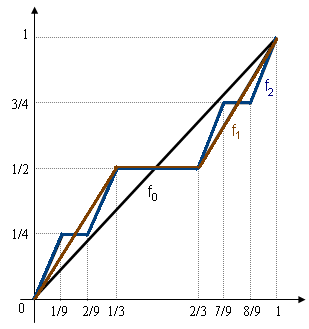
\includegraphics[width=0.4\textwidth]{diablo.png}
    \end{align*}
    Nótese que
    \begin{itemize}
        \item $f_n$ es creciente.
        \item $f_s$ es continua.
        \item Además
              \begin{align*}
                  |f_{n+1}(x) - f_n(x)| \leq \frac{1}{2^n}.
              \end{align*}
              Como $\sum_{n=1}^{\infty}{\frac{1}{2^n}} < +\infty$ entonces $\sum_{n=1}^{\infty}{(f_{n+1}(x) - f_n(x))}$ converge uniformemente.
              \begin{align*}
                  S_N(x) = sum_{n=1}^{N}{(f_{n+1}(x) - f_n(x))} = f_{N+1}(x) - f_1(x),
              \end{align*}
              por tanto, $\{f_n\}$ converge uniformemente es $[0,1]$.
    \end{itemize}
    Sea $F$ el límite uniformente de $\{f_n\}$, entonces
    \begin{itemize}
        \item $F$ es continua.
        \item $F$ es creciente.
        \item $F(1) = 1$ y $F(0) = 0$.
        \item $F'(x) = 0$ para todo $x \in [0,1] \backslash C$, donde $C$ es \textit{el conjunto de Cantor}, por tanto
              \begin{align*}
                  \int_{0}^{1}{F'(x) \ dx}  = 0.
              \end{align*}
              y $F(1) - F(0) = 1 - 0 = 1$. Por tanto
              \begin{align*}
                  \int_{0}^{1}{F'(x) \ dx}  = 0 \not = F(1) - F(0),
              \end{align*}
              es decir, no se cumple la regla de Barrow.
    \end{itemize}
    Además
    \begin{align*}
         & m_F(\mathbb{R}) = m_F([0,1]) = m_F((0,1]) = F(1) - F(0) = 1 \ \ \text{y} \\
         & m_F([0,1] \backslash C) = 0 \Longrightarrow m_F(C) = 1 \not = m(C) = 0.
    \end{align*}
    Consideremos ahora $H: [0,1] \longrightarrow \mathbb{R}$ dada por $H(x) = F(x) + x$, es claro que
    \begin{itemize}
        \item $H$ es continua.
        \item $H$ es estrictamente creciente.
        \item $H(0) = F(0) + 0 = 0$ y $H(1) = F(1) + 1 = 2$.
        \item $H([0,1]) = [0,2]$.
    \end{itemize}
    Restringiendo la imagen teneos que $H : [0,1] \longrightarrow [0,2]$ es continua y biyectiva y $H^{-1} : [0,2] \longrightarrow [0,1]$ es continua. Además, $m(H([0,1]\backslash C)) = m([0,1]\backslash C) = 1$. Calculemos ahora $m(H(C))$.
    \begin{align*}
         & [0,1] = C \cup ([0,1] \backslash C)                \\
         & H([0,1]) = H(c) \cup H([0,1] \backslash C) = [0,2] \\
    \end{align*}
    por lo que $m(H(C)) = 1$. Como tiene medida positiva, entonces existe $E \subset H(C)$ tal que $E$ no es medible-Lebesgue. Consideremos $H^{-1}(E) \subset C$. Como $m(C) = 0$ entonces $m(H^{-1}(E)) = 0$, por lo que $H^{-1}(E)$ es medible-Lebesgue, pero ¿es medible-Borel? No, porque si lo fuera, $H(H^{-1}(E)) = E$ sería medible-Borel, que no es cierto (puesto que $E$ no es medible-Lebesgue). Luego $H^{-1}(E)$ es medible-Lebesgue pero no medible-Borel.

    Adeás, $\mathcal{X}_E$ no es medible-Lebesgue, ya que
    \begin{align*}
        \mathcal{X}_E = \mathcal{X}_{H^{-1}(E)}(H^{-1}(x)) = (\mathcal{X}_{H^{-1}(E)} \circ H^{-1})(x).
    \end{align*}
\end{ejemplo}
